\documentclass[border=6pt]{standalone}
\usepackage[T1]{fontenc}
\usepackage{lmodern}
\usepackage{tikz}
\usetikzlibrary{arrows.meta,positioning,shapes.geometric,calc,fit}
\begin{document}
\hyphenpenalty=10000 \exhyphenpenalty=10000
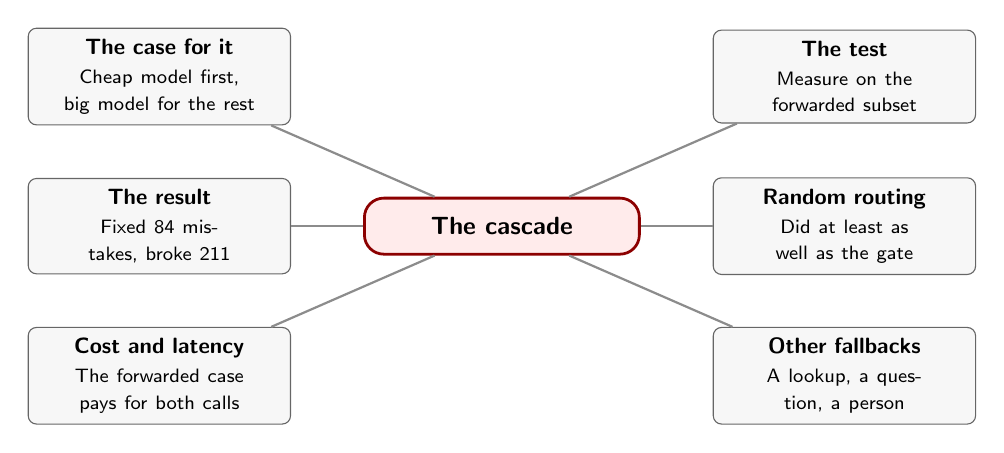
\begin{tikzpicture}[
  font=\footnotesize\sffamily,
  hub/.style={draw=red!55!black, line width=1pt, rounded corners=7pt, fill=red!8, align=center,
              text width=3cm, inner sep=7pt, font=\bfseries\small\sffamily},
  br/.style={draw=black!60, rounded corners=3pt, fill=black!3, align=center,
             text width=3.05cm, inner sep=4pt, minimum height=1.05cm},
  edge/.style={draw=black!45, line width=0.8pt}
]
\node[hub] (hub) at (0,0) {The cascade};
\node[br] (b0) at (-4.35,1.90) {\textbf{The case for it}\\[1pt]{\scriptsize Cheap model first, big model for the rest}};
\draw[edge] (hub) -- (b0);
\node[br] (b1) at (4.35,1.90) {\textbf{The test}\\[1pt]{\scriptsize Measure on the forwarded subset}};
\draw[edge] (hub) -- (b1);
\node[br] (b2) at (-4.35,0.00) {\textbf{The result}\\[1pt]{\scriptsize Fixed 84 mistakes, broke 211}};
\draw[edge] (hub) -- (b2);
\node[br] (b3) at (4.35,0.00) {\textbf{Random routing}\\[1pt]{\scriptsize Did at least as well as the gate}};
\draw[edge] (hub) -- (b3);
\node[br] (b4) at (-4.35,-1.90) {\textbf{Cost and latency}\\[1pt]{\scriptsize The forwarded case pays for both calls}};
\draw[edge] (hub) -- (b4);
\node[br] (b5) at (4.35,-1.90) {\textbf{Other fallbacks}\\[1pt]{\scriptsize A lookup, a question, a person}};
\draw[edge] (hub) -- (b5);
\end{tikzpicture}
\end{document}
